\documentclass[tikz,border=0pt]{standalone}
\usepackage{xcolor}
\usetikzlibrary{calc}
% Palette: Sam_Comm_final.png by eye (vagrancy repository).
\definecolor{ink}{HTML}{3B2340}
\definecolor{dark}{HTML}{4A3357}
\definecolor{darkhi}{HTML}{5E4A6E}
\definecolor{sky}{HTML}{EFC46A}
\definecolor{skyhi}{HTML}{F5DA92}
\definecolor{skylow}{HTML}{E9B060}
\definecolor{cloud}{HTML}{F2D58A}
\definecolor{wallA}{HTML}{E88A73}
\definecolor{wallB}{HTML}{EE9F7E}
\definecolor{wallC}{HTML}{E47A7E}
\definecolor{wallD}{HTML}{F0B07E}
\definecolor{wallE}{HTML}{D9765F}
\definecolor{wallF}{HTML}{E99A8A}
\definecolor{greenA}{HTML}{8DBB7E}
\definecolor{greenB}{HTML}{6FA77A}
\definecolor{greenC}{HTML}{A9C97F}
\definecolor{greenD}{HTML}{5E9C6A}
\definecolor{window}{HTML}{F6E7A0}
\definecolor{windark}{HTML}{8C5A64}
\definecolor{plum}{HTML}{8A5A9E}
\definecolor{plumhi}{HTML}{A77BB8}
\definecolor{lilac}{HTML}{D9C3E0}
\definecolor{coral}{HTML}{E47A7E}
\definecolor{coraldk}{HTML}{C85F65}
\definecolor{orange}{HTML}{F26B38}
\definecolor{salmon}{HTML}{F4BE9C}
\definecolor{gold}{HTML}{F2B53A}
\definecolor{golddk}{HTML}{D9962A}
\definecolor{butter}{HTML}{F5DA92}
\definecolor{cream}{HTML}{FFF4E0}
\definecolor{paper}{HTML}{F6E7C4}
\definecolor{sage}{HTML}{8DBB7E}
\definecolor{sagedk}{HTML}{6FA77A}
\definecolor{forest}{HTML}{5E9C6A}
\definecolor{mint}{HTML}{C5E0B4}
\definecolor{teal}{HTML}{5FA8A0}
\definecolor{glass}{HTML}{A9D3C9}
\definecolor{glassdk}{HTML}{7FB7B0}
\definecolor{pink}{HTML}{F2A7B5}
\definecolor{rosewall}{HTML}{F3B7A8}
\definecolor{steel}{HTML}{C8C2B4}
\definecolor{steeldk}{HTML}{8D9A93}
\definecolor{metal}{HTML}{8D9A93}
\definecolor{wood}{HTML}{B9835A}
\definecolor{wooddk}{HTML}{8E5E3C}
\definecolor{tan}{HTML}{E2BD8C}
\definecolor{paving}{HTML}{E2BD8C}
\definecolor{ground}{HTML}{D3A77D}
% One ink for every outline.
\newcommand{\Ink}{1.3pt}
\tikzset{inked/.style={draw=ink, line width=\Ink, line join=round, line cap=round}}
% Picture units: 0.4 mm, y counted downward (hence the negative y unit).
\tikzset{x=0.4mm, y=-0.4mm}
\begin{document}
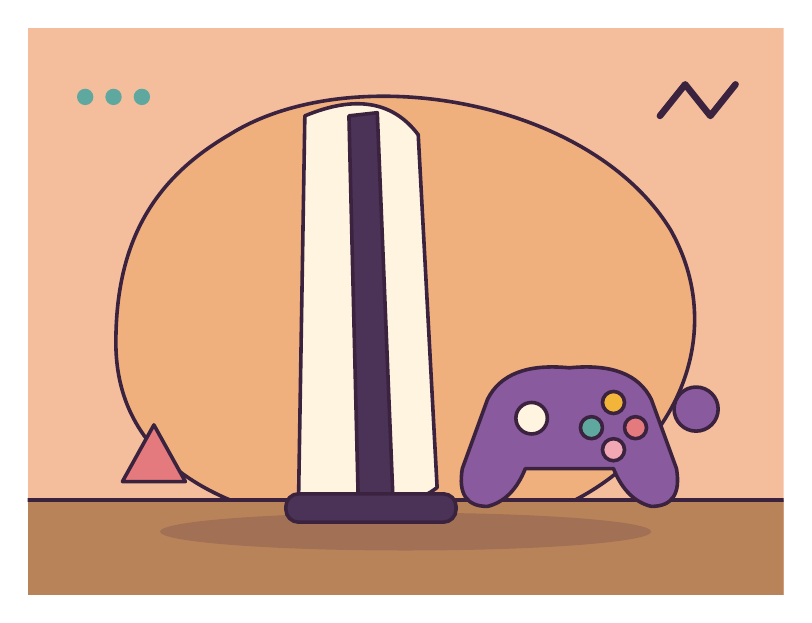
\begin{tikzpicture}
\clip (0,0) rectangle (240,180);
% background: wall, floor, blob, confetti
\fill[salmon] (0,0) rectangle (240,180);
\filldraw[inked,fill=wallD] (64,34) .. controls (102,10) and (178,22) .. (204,64) .. controls (228,106) and (194,158) .. (134,160) .. controls (82,162) and (28,148) .. (28,100) .. controls (28,68) and (40,48) .. (64,34) -- cycle;
\filldraw[inked,fill=plum] (212.23,121.1) circle [radius=7];
\draw[ink, line width=2.4pt, line cap=round, line join=round] (200.75,28.01) -- (208.75,18.01) -- (216.75,28.01) -- (224.75,18.01);
\filldraw[inked,fill=coral] (30.08,144.12) -- (40.08,126.12) -- (50.08,144.12) -- cycle;
\foreach \dx in {0,9,18} \fill[teal] (18.26+\dx,21.98) circle [radius=2.6];
\fill[wood] (0,150) rectangle (240,180);
\draw[ink, line width=1.3pt, line cap=round, line join=round] (0,150) -- (240,150);
\fill[ink, opacity=0.18] (120,160) ellipse [x radius=78, y radius=6];
% the item
\filldraw[inked,fill=cream] (88,28) .. controls (104,21.33) and (116,23.33) .. (124,34) -- (130,146) .. controls (119.33,154) and (104.67,155.33) .. (86,150) -- cycle;
\filldraw[inked,fill=dark] (102,28) -- (111,27) -- (116,150) -- (105,152) -- cycle;
\filldraw[inked,fill=dark,rounded corners=1.6mm] (82,148) rectangle (136,157);
\filldraw[inked,fill=plum] (146,118) .. controls (150,110) and (158.67,106.67) .. (172,108) .. controls (185.33,106.67) and (194,110) .. (198,118) -- (206,140) .. controls (207.33,148) and (204.67,152) .. (198,152) .. controls (192.67,150.67) and (188.67,146.67) .. (186,140) -- (158,140) .. controls (155.33,146.67) and (151.33,150.67) .. (146,152) .. controls (139.33,152) and (136.67,148) .. (138,140) -- cycle;
\filldraw[inked,fill=cream] (160,124) circle [radius=5];
\filldraw[inked,fill=gold] (186,119) circle [radius=3.5];
\filldraw[inked,fill=coral] (193,127) circle [radius=3.5];
\filldraw[inked,fill=teal] (179,127) circle [radius=3.5];
\filldraw[inked,fill=pink] (186,134) circle [radius=3.5];
\end{tikzpicture}
\end{document}
